\newpage
\section{Results}

\subsection{Training}

For each of the models, a number of episodes and batch size was chosen such that the model would converge to a stable policy within a reasonable time period ($t \leq 1h$). In practice this resulted in the parameters defined in table \ref{tab:training-parameters}. In this table, a distinction between a `deep' and `shallow' network is made. The deep network consists of the input layer, three layers of 512 neurons each and the output layer (5 layers total). The shallow network consists of the input layer, a single layer of 128 neurons and the output layer (3 layers total). The accuracy of both models is compared.

\begin{table}[H]
    \begin{tabular}{|l|l|l|p{3cm}|l|p{2.2cm}|}
        \hline
        \multicolumn{6}{|c|}{Training parameters} \\
        \hline
        Model & Episodes & Batch size & \# FC layers & $\epsilon$-decay & Learning rate $\alpha$\\
        \hline
        Single transition & 1000 & 64 & \emph{Deep:} [512, 512, 512]\linebreak\emph{Shallow:} [128] & 0.9995 & \emph{Deep:} $0.0001$\linebreak\emph{Shallow:} $0.001$\\
        \hline
        Success fail & 4000 & 64 & \emph{Deep:} [512, 512, 512]\linebreak\emph{Shallow:} [128] & 0.9995 & \emph{Deep:} $0.0001$\linebreak\emph{Shallow:} $0.001$\\
        \hline
        Safe risk & 4000 & 64 & \emph{Deep:} [512, 512, 512]\linebreak\emph{Shallow:} [128] & 0.9995 & \emph{Deep:} $0.0001$\linebreak\emph{Shallow:} $0.001$\\
        \hline
        EAJS & 500 & 128 & \emph{Deep:} [512, 512, 512]\linebreak\emph{Shallow:} [128] & 0.9995 & \emph{Deep:} $0.0001$\linebreak\emph{Shallow:} $0.001$\\
        \hline
        Consensus & 500 & 128 & \emph{Deep:} [512, 512, 512]\linebreak\emph{Shallow:} [128] & 0.9995 & \emph{Deep:} $0.0001$\linebreak\emph{Shallow:} $0.001$\\
        \hline
    \end{tabular}
    \caption{Training parameters for each model.}
    \label{tab:training-parameters}
\end{table}

Each of the models were trained on a single NVIDIA GeForce GTX 1650 Mobile laptop GPU. Execution time varied from approach, but was generally around $2 - 5m$ when utilizing a Q-table and around $30 - 45m$ when encoding the action-space as the input to the neural network for the 5-layer deep network. For the 3-layered shallow network the timing was $1 - 2m$ and $20 - 25m$ respectively. This difference in execution time between the two approaches is due to the difference in how the action-space is encoded. In the Q-table approach, the action-space is encoded as a sparse representation in the output layer. Whereas in the input layer approach, the size of the input layer is proportional to the size of the action-space. The former method produces an answer to $Q(s, a)$ for all actions $a$ given a state $s$. The latter method produces a single $Q(s, a)$ given a specific action $a$ and state $s$. Therefore, to find the optimal Q-value, multiple queries must be made to the network instead of one. This results in a slower learning process. For some models, the Q-table approach was not converging to the correct answer, and was therefore not considered as a viable approach for more complex variants of said model.

\newpage
\subsection{Sigle-transition model}

The first model to be evaluated is the single-transition model. The results of the evaluation are shown in figure \ref{fig:single-transition-R1-q}. The results show that all models converge to the same policy at a comparable number of episodes ($k \approx 140$ epsiodes). Noteworthy is the absense of convergence for the first $64$ number of episodes, this is due to the model being trained on a batch size of $64$. This means that the model is not trained until the first batch of $64$ episodes has been completed. This is also the reason why the first $64$ episodes are not shown in the figure.

\begin{figure}
    \centering
    \begin{subfigure}[b]{0.9\textwidth}
        \centering
        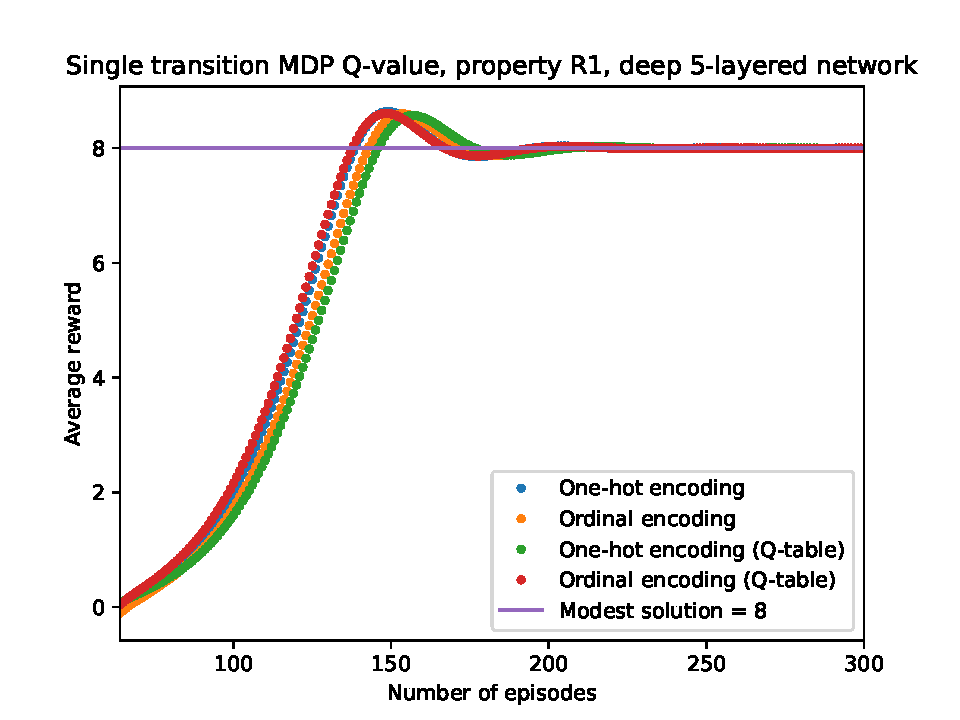
\includegraphics[width=\textwidth]{plot/single-transition-R1-q.pdf}
        \caption{Single-transition model trained on the deep network. All models converge to the same policy at a comparable number of episodes ($k \approx 140$ epsiodes).}
        \label{fig:single-transition-R1-deep-q}
    \end{subfigure}
    \vfill
    \begin{subfigure}[b]{0.9\textwidth}
        \centering
        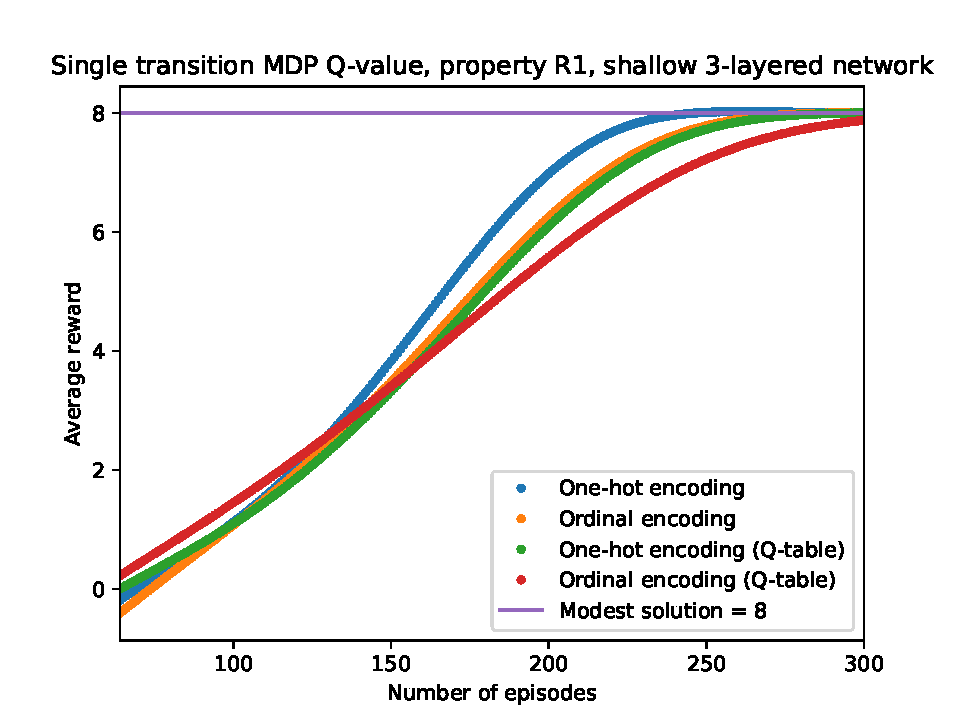
\includegraphics[width=\textwidth]{plot/single-transition-R1-fc128-q.pdf}
        \caption{Single-transition model trained on the shallow network. All models converge to the same policy starting at $k = 220$ episodes. The one-hot encoding is sightly faster than the ordinal encoding.}
        \label{fig:single-transition-R1-shallow-q}
    \end{subfigure}
    \caption{Single-transition model trained on the deep and shallow network.}
    \label{fig:single-transition-R1-q}
\end{figure}

Figure \ref{fig:single-transition-R1-q} shows that the model is able to learn the optimal policy for the single-transition model, and therefore implies that the parameters of Q-learning are set correctly. If at this stadium the model was not able to learn the optimal policy, the underlying code would be checked for errors. The 5-layered deep model converges after overshooting slightly to $r \approx 8.6$ and then converging to $r = 8$. The shallow model takes longer to converge than the deep model, even though the learning rate is $10 \times$ higher. This is due to the shallow model having fewer neurons, and therefore the weights get multiplied less.

\subsection{Success-fail model}

The second model to be evaluated is the success-fail model. The results of the evaluation are shown in figure \ref{fig:success-fail-R1-q}. In this model, which is a slightly more complex variant of the initial model as it includes a fail state, the model is not able to converge to the optimal policy in a stable manner.

\begin{figure}
    \centering
    \begin{subfigure}[b]{0.9\textwidth}
        \centering
        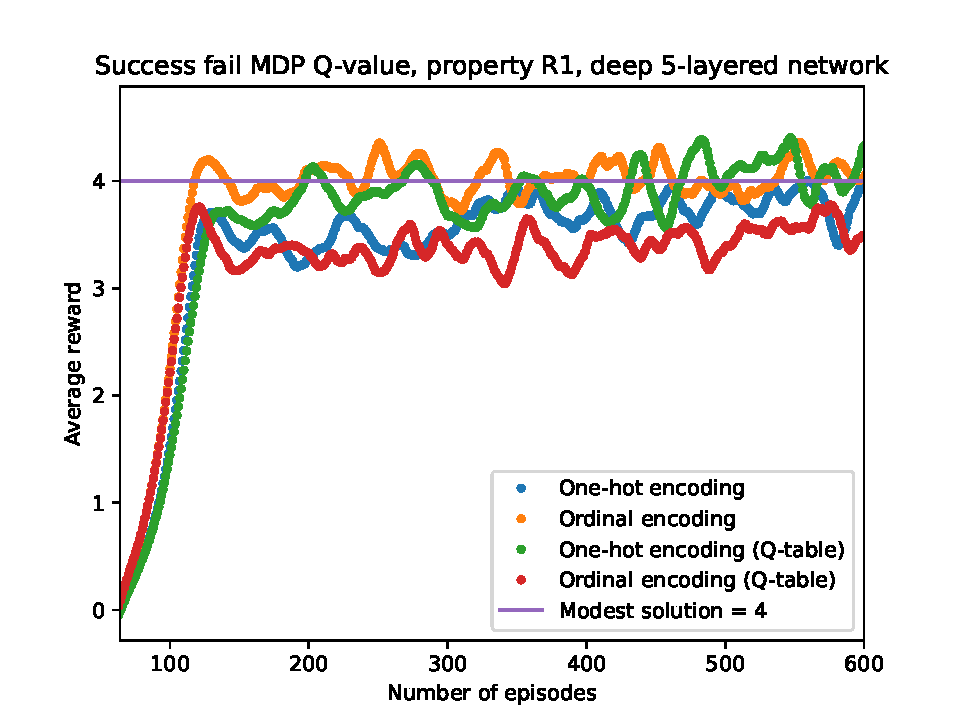
\includegraphics[width=\textwidth]{plot/success-fail-R1-q.pdf}
        \caption{Success-fail model trained on the deep network. All models fail to converge completely, and oscillate around the solution.}
        \label{fig:success-fail-R1-deep-q}
    \end{subfigure}
    \vfill
    \begin{subfigure}[b]{0.9\textwidth}
        \centering
        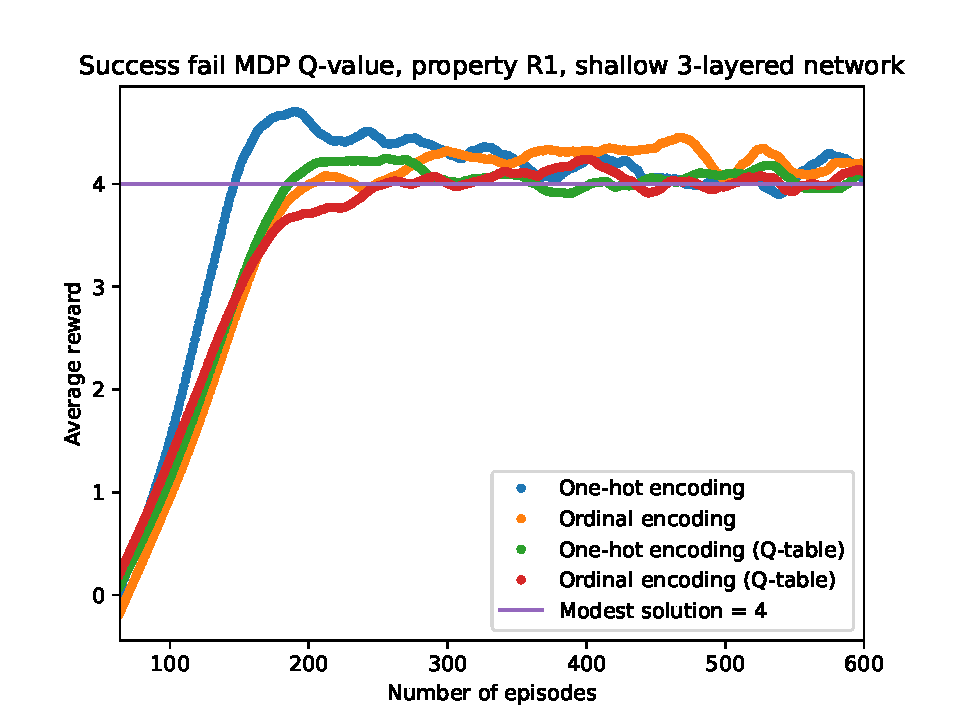
\includegraphics[width=\textwidth]{plot/success-fail-R1-fc128-q.pdf}
        \caption{Success-fail model trained on the shallow network. All models fail to converge completely, and oscillate around the solution. However less so than in the deep network of figure \ref{sub@fig:success-fail-R1-deep-q}. The one-hot Q-table encoding performs best in this scenario.}
        \label{fig:success-fail-R1-shallow-q}
    \end{subfigure}
    \caption{Success-fail model trained on the deep and shallow network.}
    \label{fig:success-fail-R1-q}
\end{figure}

Figure \ref{fig:success-fail-R1-q} shows that the model is being pulled towards either of the reward states (i.e., succes $r = 8$ or fail $r = 0$), and is not able to correctly identify the solution as being $r = \frac{8 + 0}{2} = 4$. When oscillating around the solution, the model is displaced the least, and as such this is the resulting average reward of the model. This result clearly demonstates that for each of the approaches, a trivial model such as a two-transition system is not able to be learned by the model. There are no clear differences between he ordinal and one-hot encoding, as well as the Q-table and input layer approach. In this particular case, the Q-table ordinal encoding performs the worst, but this could be explained by the random initialization of the Q-table. Repetition of the experiment could result in a different outcome, but remains close to the other approaches.

\subsection{Safe-risk model}

The third model to be evaluated is the safe-risk model. The results of the evaluation are shown in figure \ref{fig:safe-risk-R1-q}. In this model, a choice is introduced between a safe and a risky action. The safe action results in a reward of $r = 2$ at a $90$ percent probability, whereas the risky action results in a reward of $r = 8$ at a $50$ percent probability. The optimal policy is therefore to always choose the risky action. The results show that the model is able to learn the optimal policy in a stable manner.

\begin{figure}
    \centering
    \begin{subfigure}[b]{0.9\textwidth}
        \centering
        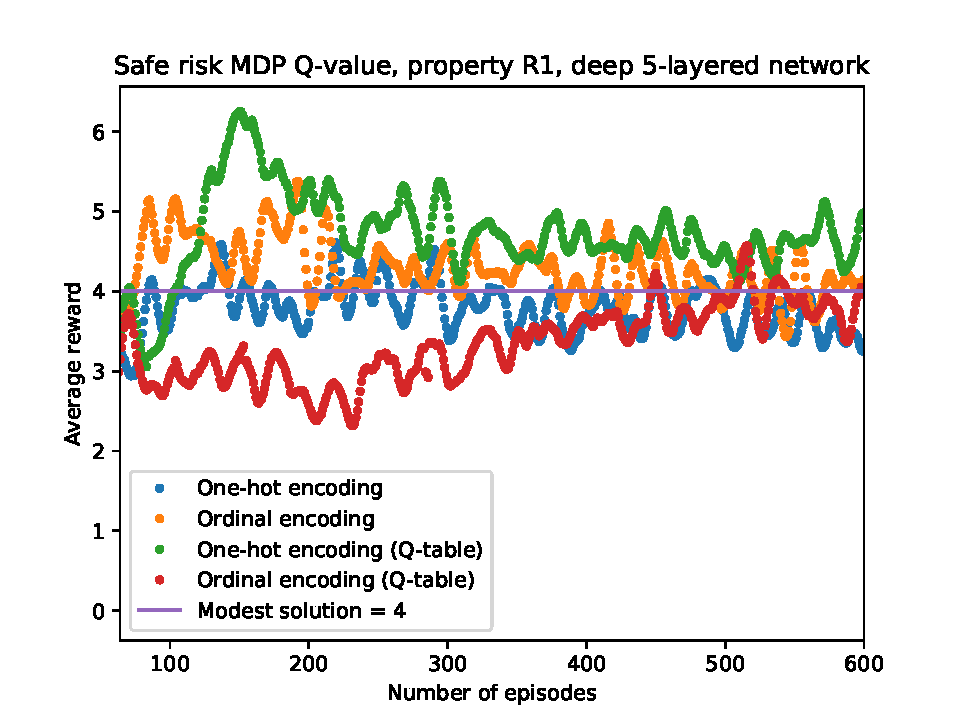
\includegraphics[width=\textwidth]{plot/safe-risk-R1-q.pdf}
        \caption{Success-fail model trained on the deep network. All models fail to converge completely, and oscillate around the solution.}
        \label{fig:safe-risk-R1-deep-q}
    \end{subfigure}
    \vfill
    \begin{subfigure}[b]{0.9\textwidth}
        \centering
        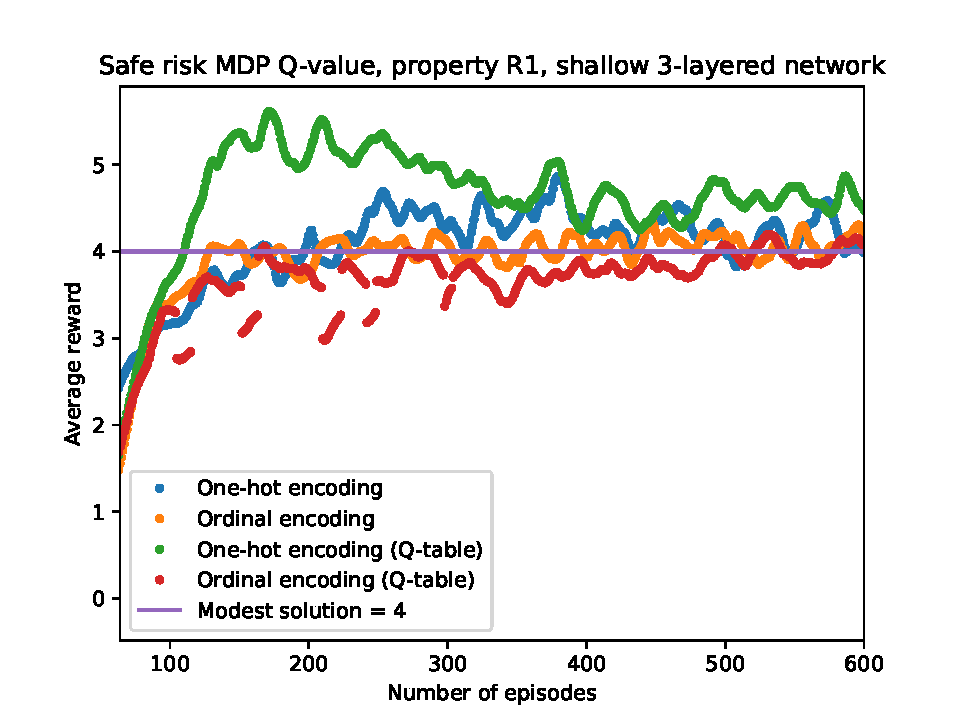
\includegraphics[width=\textwidth]{plot/safe-risk-R1-fc128-q.pdf}
        \caption{Success-fail model trained on the shallow network. All models fail to converge completely, and oscillate around the solution. However less so than in the deep network of figure \ref{sub@fig:safe-risk-R1-deep-q}. The one-hot input-layer encoding performs best in this scenario.}
        \label{fig:safe-risk-R1-shallow-q}
    \end{subfigure}
    \caption{Safe-risk model trained on the deep and shallow network.}
    \label{fig:safe-risk-R1-q}
\end{figure}

Figure \ref{fig:safe-risk-R1-q} shows all models converging around the solution of $r = 4$, however not in a stable manner. The one-hot input-layer encoding approach is very close to the correct answer around $k = 150$ epsiodes, but diverges to a lower value for $r$ as the model continues to train. The one-hot and ordinal Q-table approaches deviate the greatest from the actual solution before $k = 400$ episodes, but converge more near $k = 600$ episodes. The ordinal input-layer approach fluctuates between $r = 4$ and $r = 5$ for the majority of the training period, but converges to $r = 4$ near $k = 600$ episodes. The one-hot Q-table encoding approaches the correct solution of $r = 4$ but for $k \leq 300$ episodes undershoots to $r \approx 3$. This sudden change of expected reward can be the result of the network giving a relatively high weight to a neuron, and suddenly changing it as the result of exploring the model. These outlyers are corrected further along the training process and this does not occur for $k > 300$ episodes.

\subsection{Energy-aware Job Scheduling QComp model}

\subsubsection*{N = 2}
The first QComp model is Energy-aware Job Scheduling for the following parameters: $N = 2$, $energy\_capacity = 100$ and $B = 5$.

\begin{figure}
    \centering
    \begin{subfigure}[b]{0.9\textwidth}
        \centering
        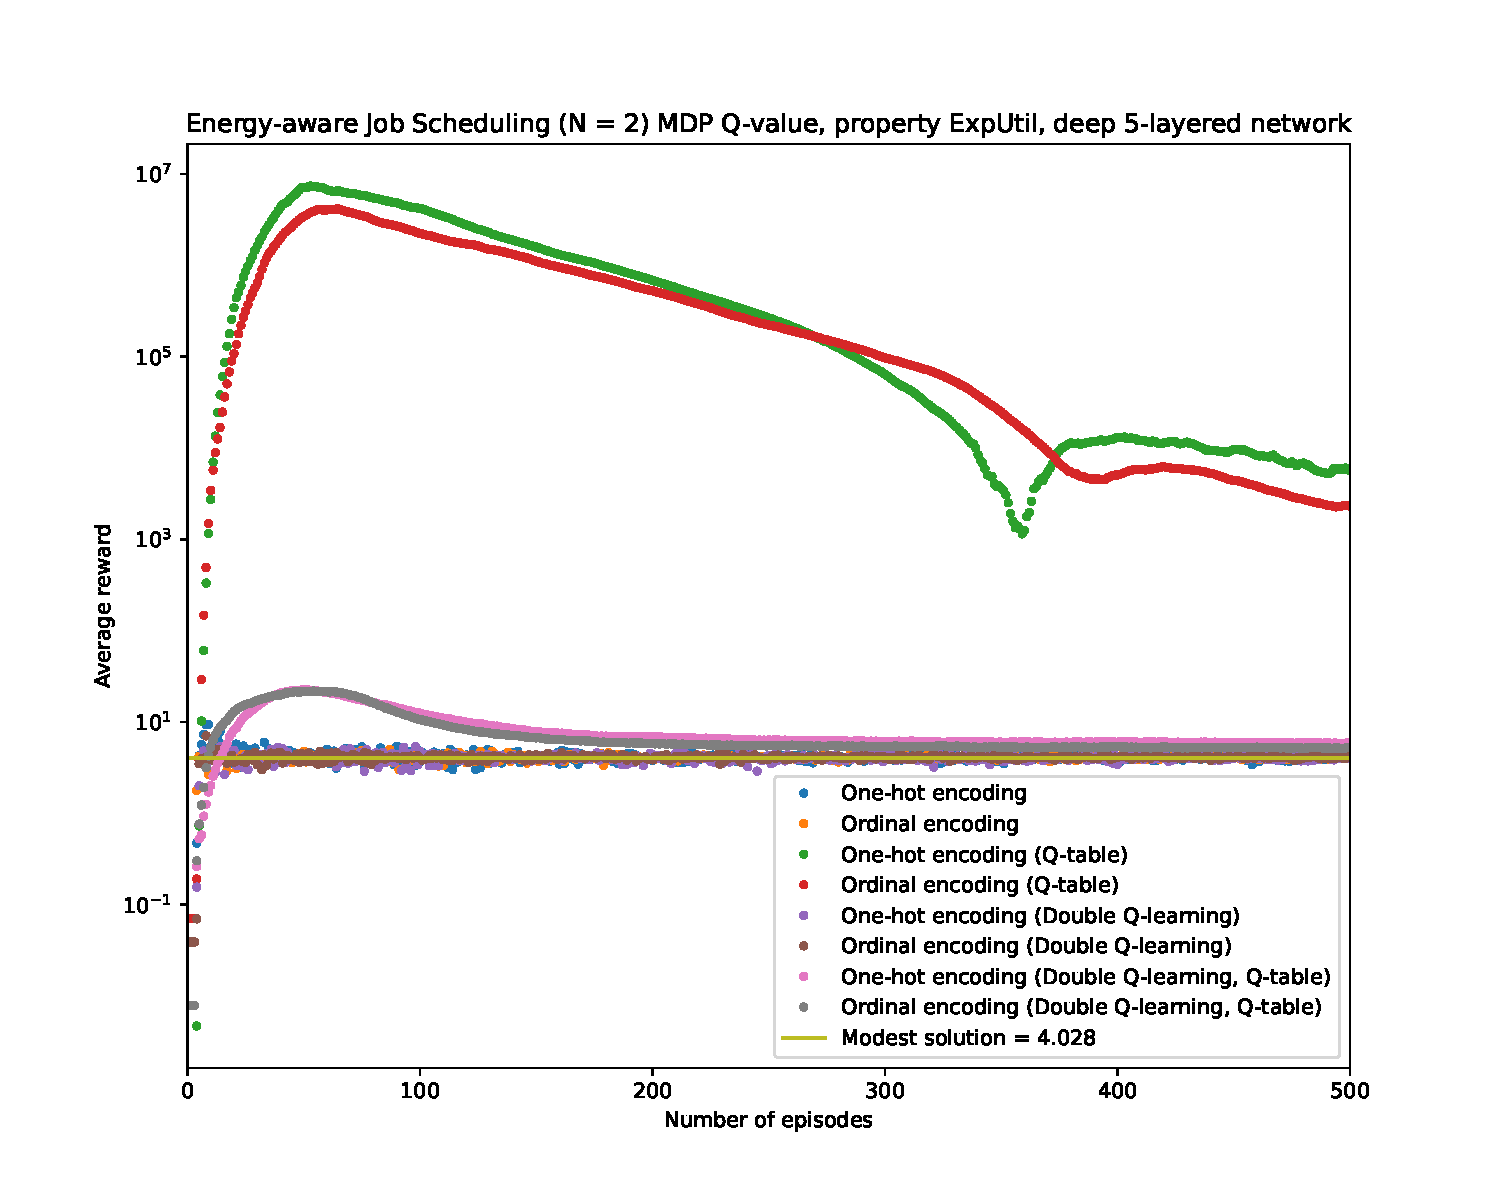
\includegraphics[width=\textwidth]{plot/eajs.2-ExpUtil-q.pdf}
        \caption{EAJS trained on the deep model.}
        \label{fig:eajs.2-ExpUtil-deep-q}
    \end{subfigure}
    \vfill
    \begin{subfigure}[b]{0.9\textwidth}
        \centering
        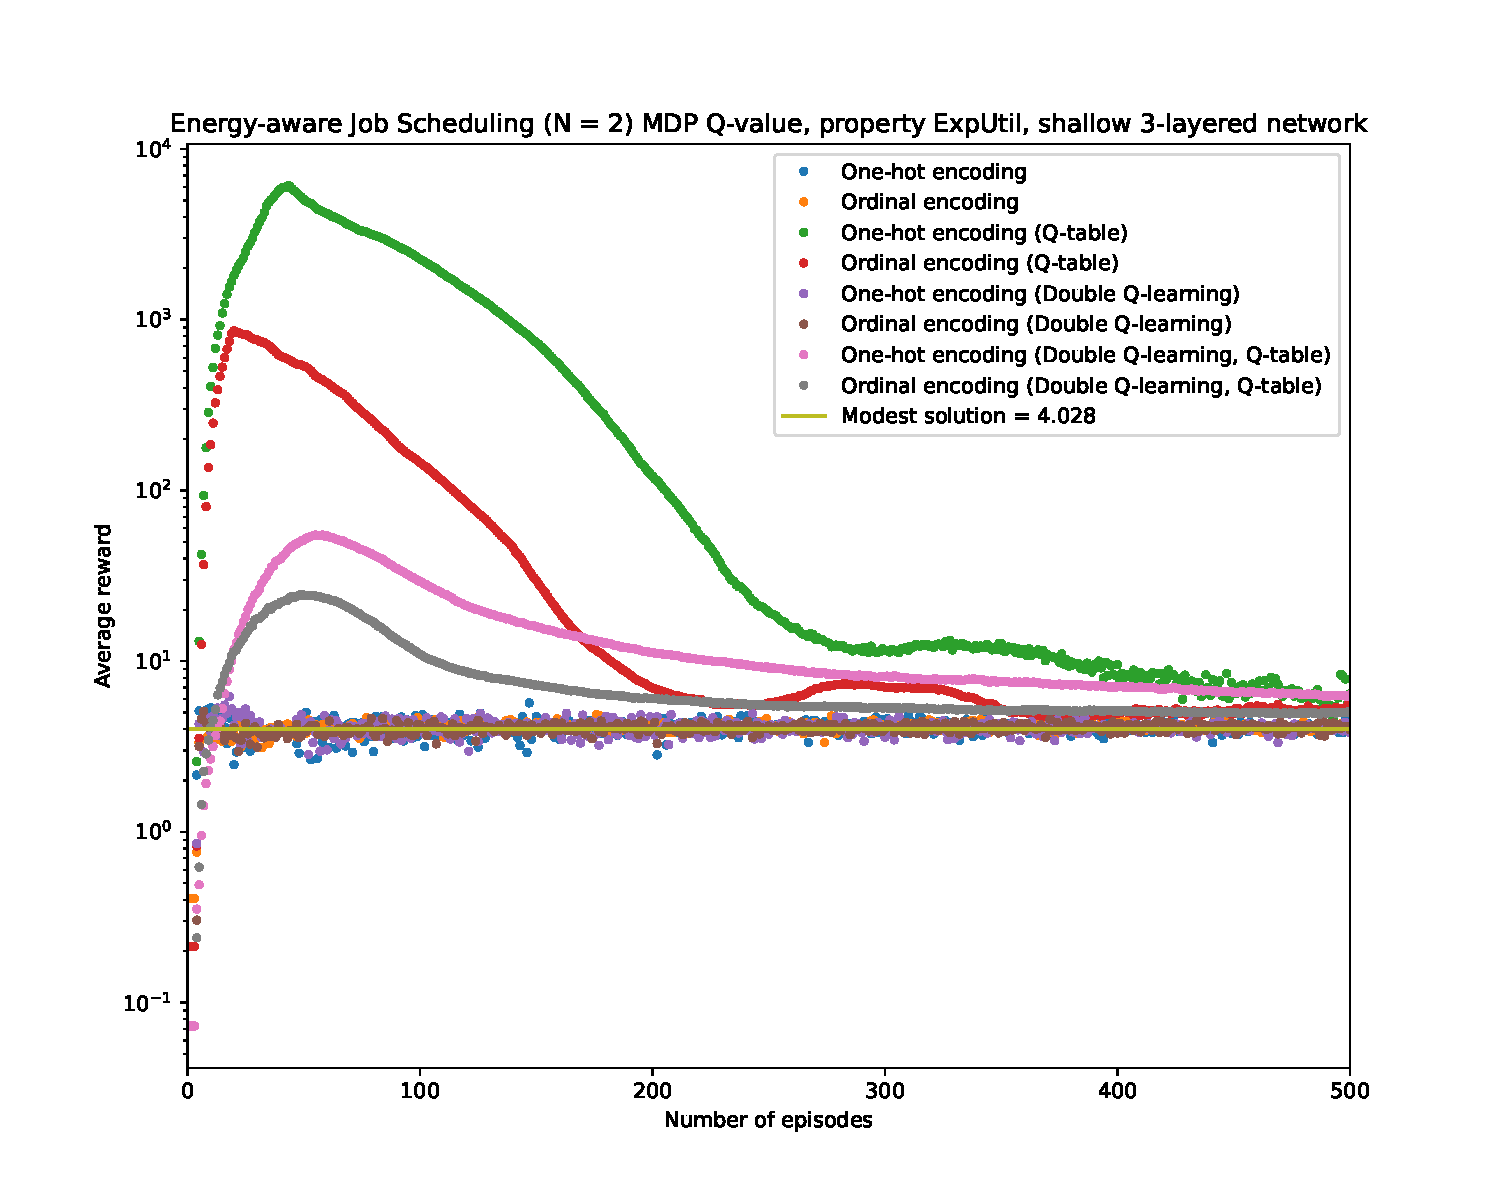
\includegraphics[width=\textwidth]{plot/eajs.2-ExpUtil-fc128-q.pdf}
        \caption{EAJS trained on the shallow model. In this shallow model, the Q-table encodings explode less in value than in figure \ref{sub@fig:eajs.2-ExpUtil-deep-q}. This is due the network having fewer neurons, and therefore the weights are multiplied less.}
        \label{fig:eajs.2-ExpUtil-shallow-q}
    \end{subfigure}
    \caption{Energy-aware Job Scheduling QComp model trained on the deep and shallow network. All Q-table approaches fail to converge to the optimal policy, whilst all input-layer encoded method fluctuate around the solution of $r = 4.028$.}
    \label{fig:eajs.2-ExpUtil-q}
\end{figure}

Figure \ref{fig:eajs.2-ExpUtil-q} shows that the Q-table approach tends to explode in value. In these figures the outlyers (Q-table encoding results) are most predominant. Therefore the Q-table approach was not utilized for the more complex variant of this model.

\subsubsection*{N = 4}
Energy-aware Job Scheduling was also solved for the following parameters: $N = 4$, $energy\_capacity = 200$ and $B = 9$. This is a more complex variant of the previous model, and therefore requires a more complex neural network to learn the optimal policy.

\begin{figure}
    \centering
    \begin{subfigure}[b]{0.9\textwidth}
        \centering
        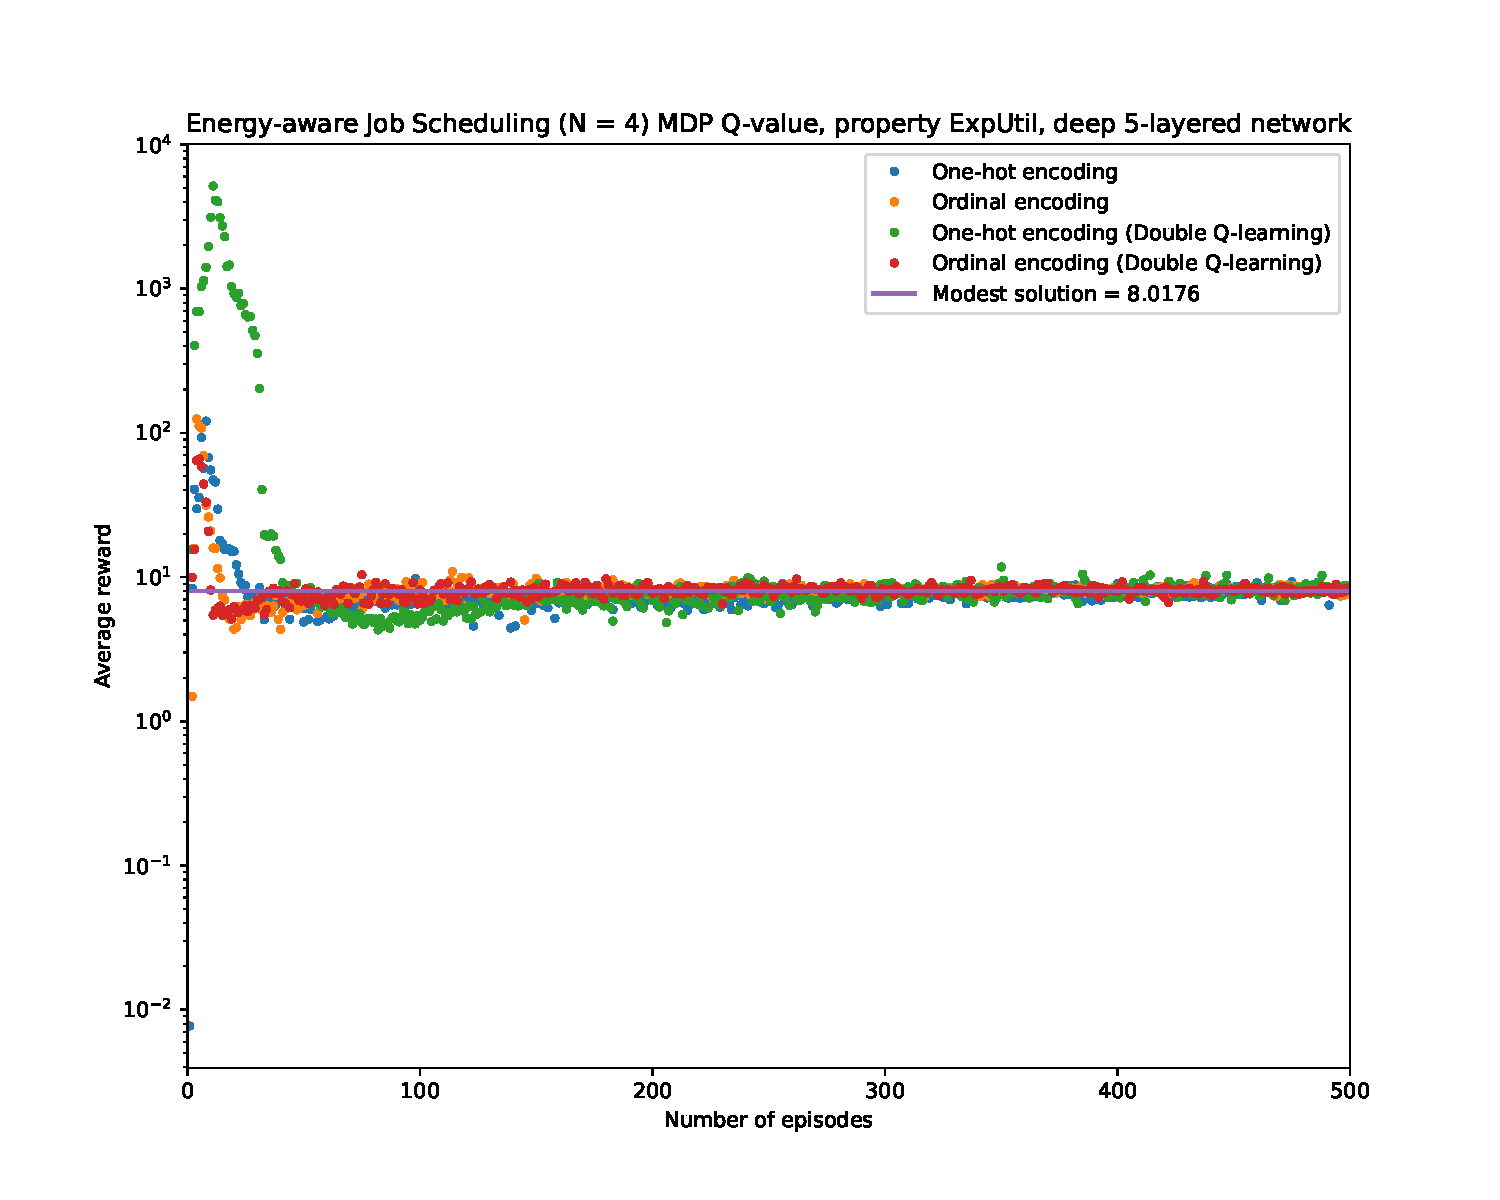
\includegraphics[width=\textwidth]{plot/eajs.4-ExpUtil-q.pdf}
        \caption{EAJS trained on the deep model. In this model, all approaches converge to the correct solution of $r = 8.0176$. Noteworthy is the Double-Q learning method is the slowest to converge, in particular the one-hot variant.}
        \label{fig:eajs.4-ExpUtil-deep-q}
    \end{subfigure}
    \vfill
    \begin{subfigure}[b]{0.9\textwidth}
        \centering
        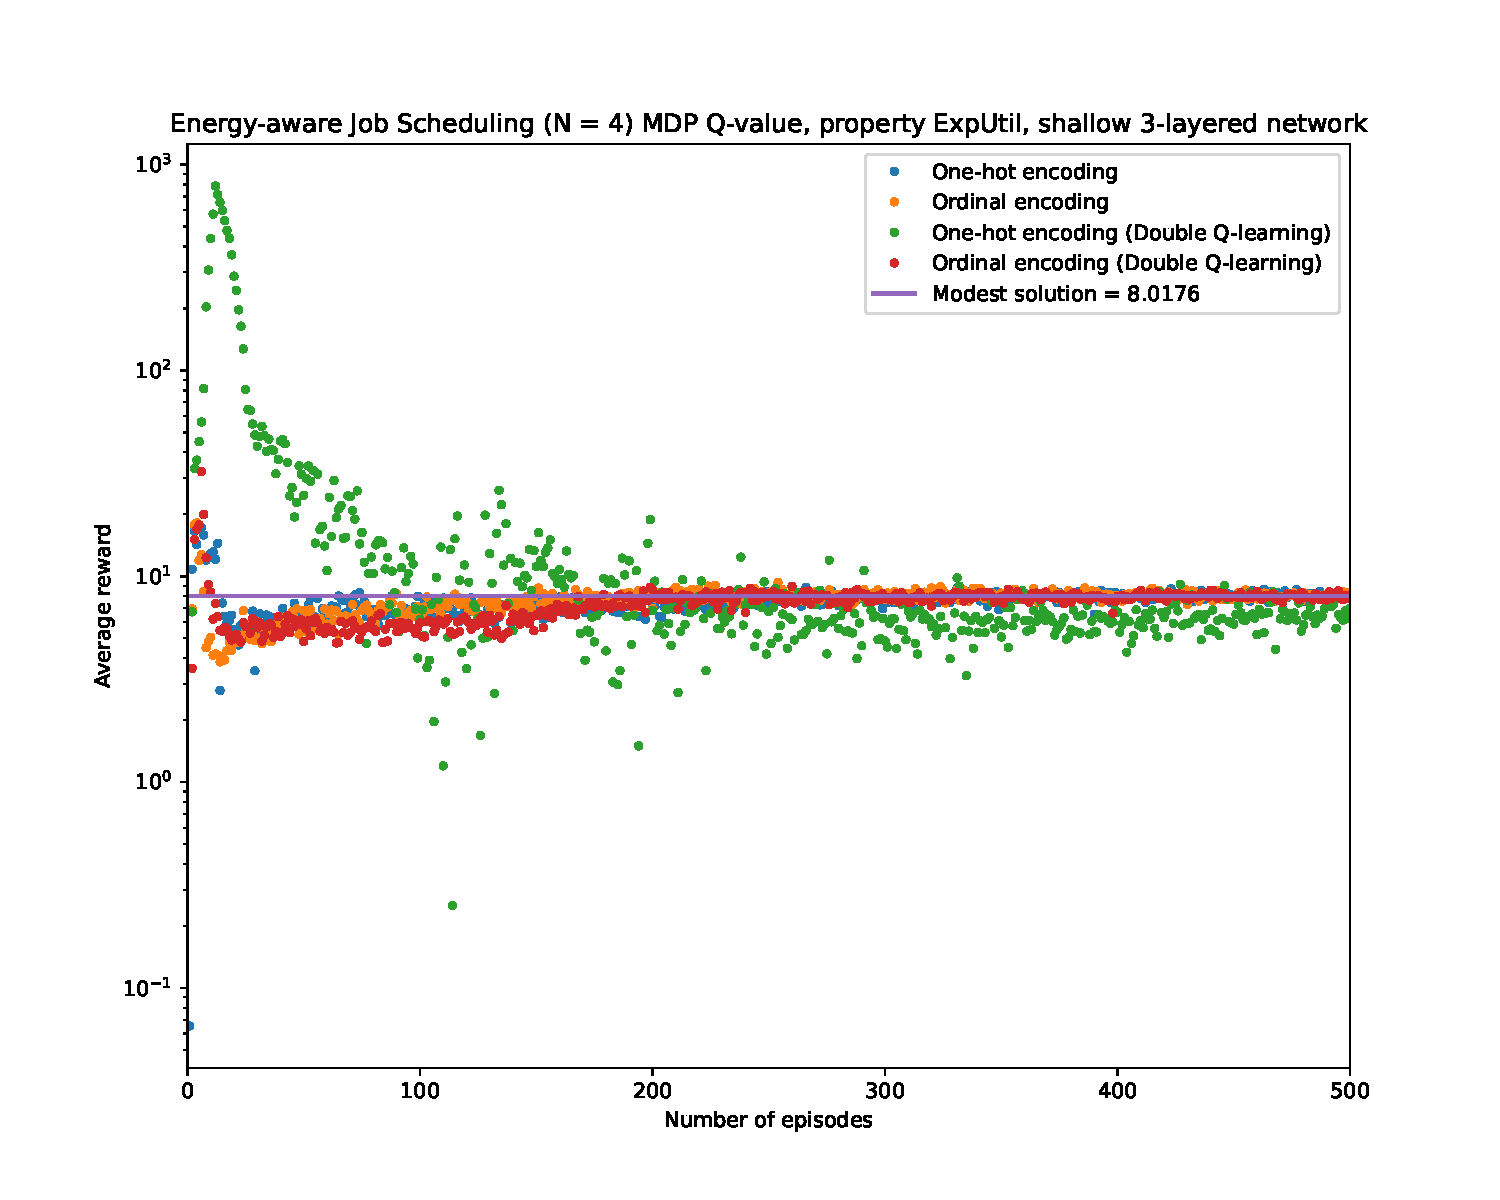
\includegraphics[width=\textwidth]{plot/eajs.4-ExpUtil-fc128-q.pdf}
        \caption{EAJS trained on the shallow model. Here, just as with the deep model in figure \ref{sub@fig:eajs.4-ExpUtil-deep-q} the one-hot encoded Double Q-learning variant is the sowest to converge, and oscillates significantly more than the other approaches.}
        \label{fig:eajs.4-ExpUtil-shallow-q}
    \end{subfigure}
    \caption{Energy-aware Job Scheduling QComp model trained on the deep and shallow network.}
    \label{fig:eajs.4-ExpUtil-q}
\end{figure}

Figure \ref{fig:eajs.4-ExpUtil-q} shows that all approaches converge to the correct solution of $r = 8.0176$. This happens relatively early in the training process at $k \approx 50$ episodes. All approaches converge, with the one-hot Double Q-learning approach converging after overshooting to $r \approx 5 \times 10^3$. It is unclear why this occurred, as the one-hot encoding and Double Q-learning approach separately do not exhibit this behaviour. It is possible that the combination of the two approaches results in this behaviour.

\subsection{Randomized Consensus Protocol}

The second QComp model is Randomized Consensus Protocol for the following parameters: $K = 2$.

\begin{figure}
    \centering
    \begin{subfigure}[b]{0.9\textwidth}
        \centering
        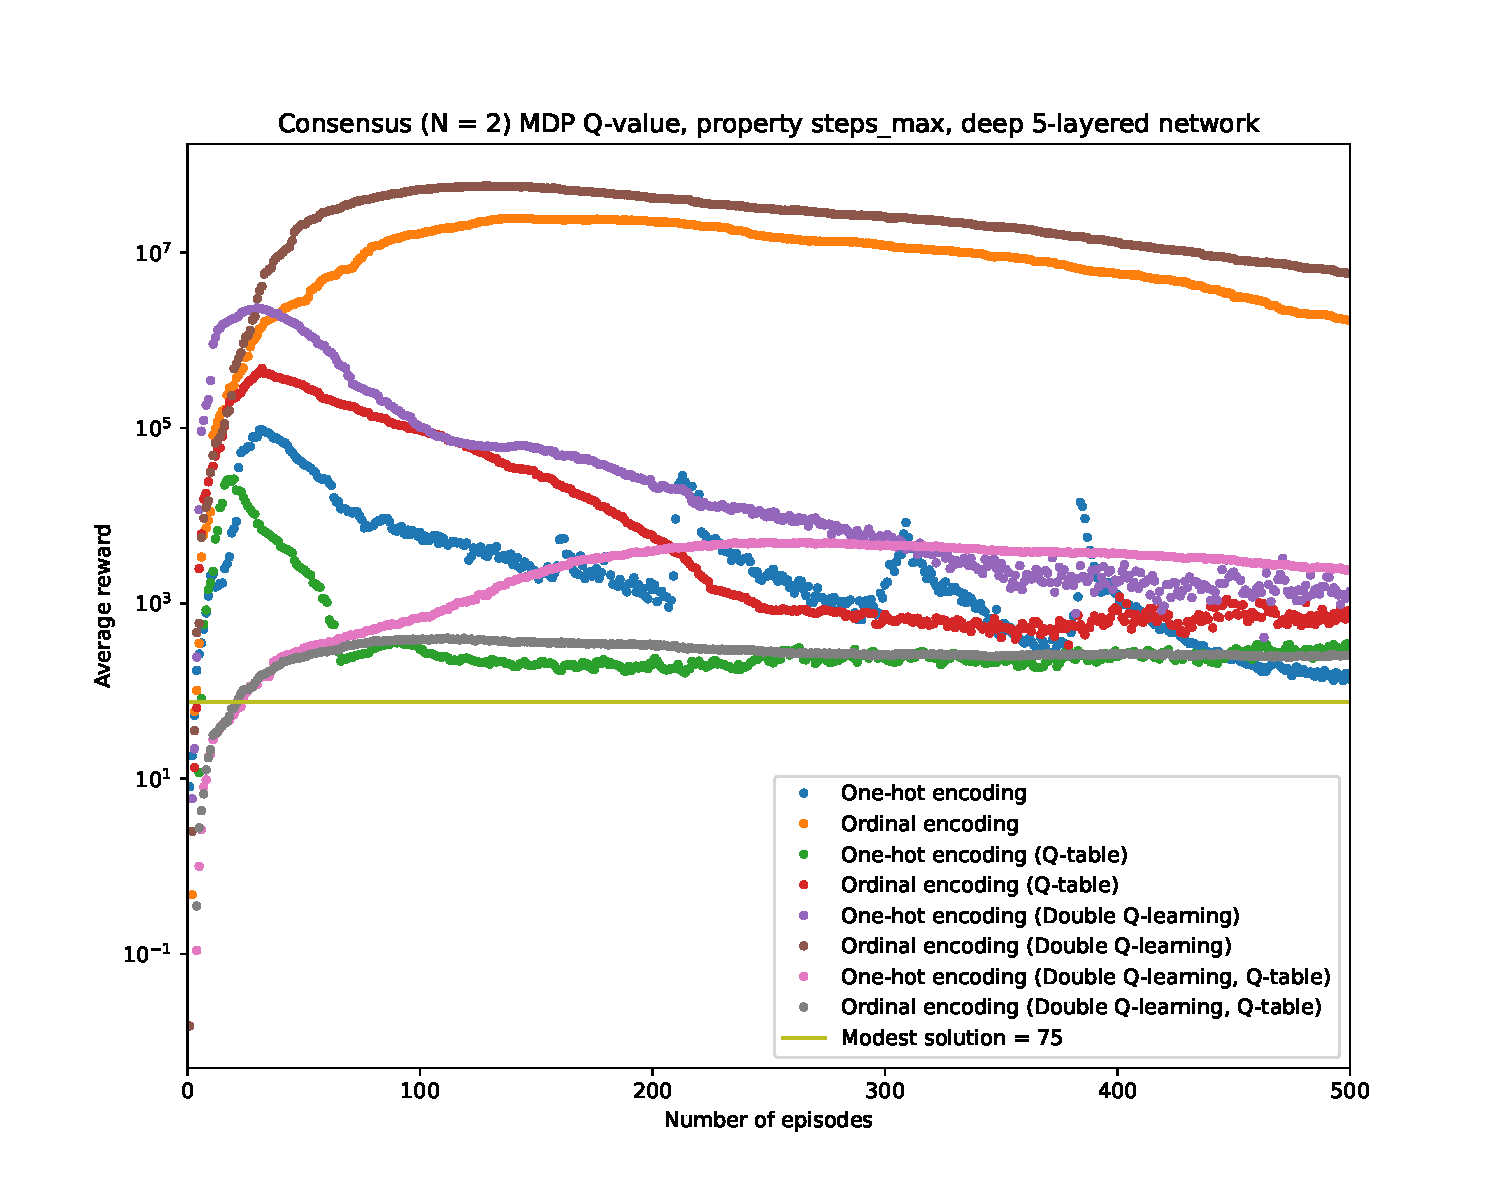
\includegraphics[width=\textwidth]{plot/consensus.2-steps_max-q.pdf}
        \caption{Consensus trained on the deep model.}
        \label{fig:consensus.2-steps_max-deep-q}
    \end{subfigure}
    \vfill
    \begin{subfigure}[b]{0.9\textwidth}
        \centering
        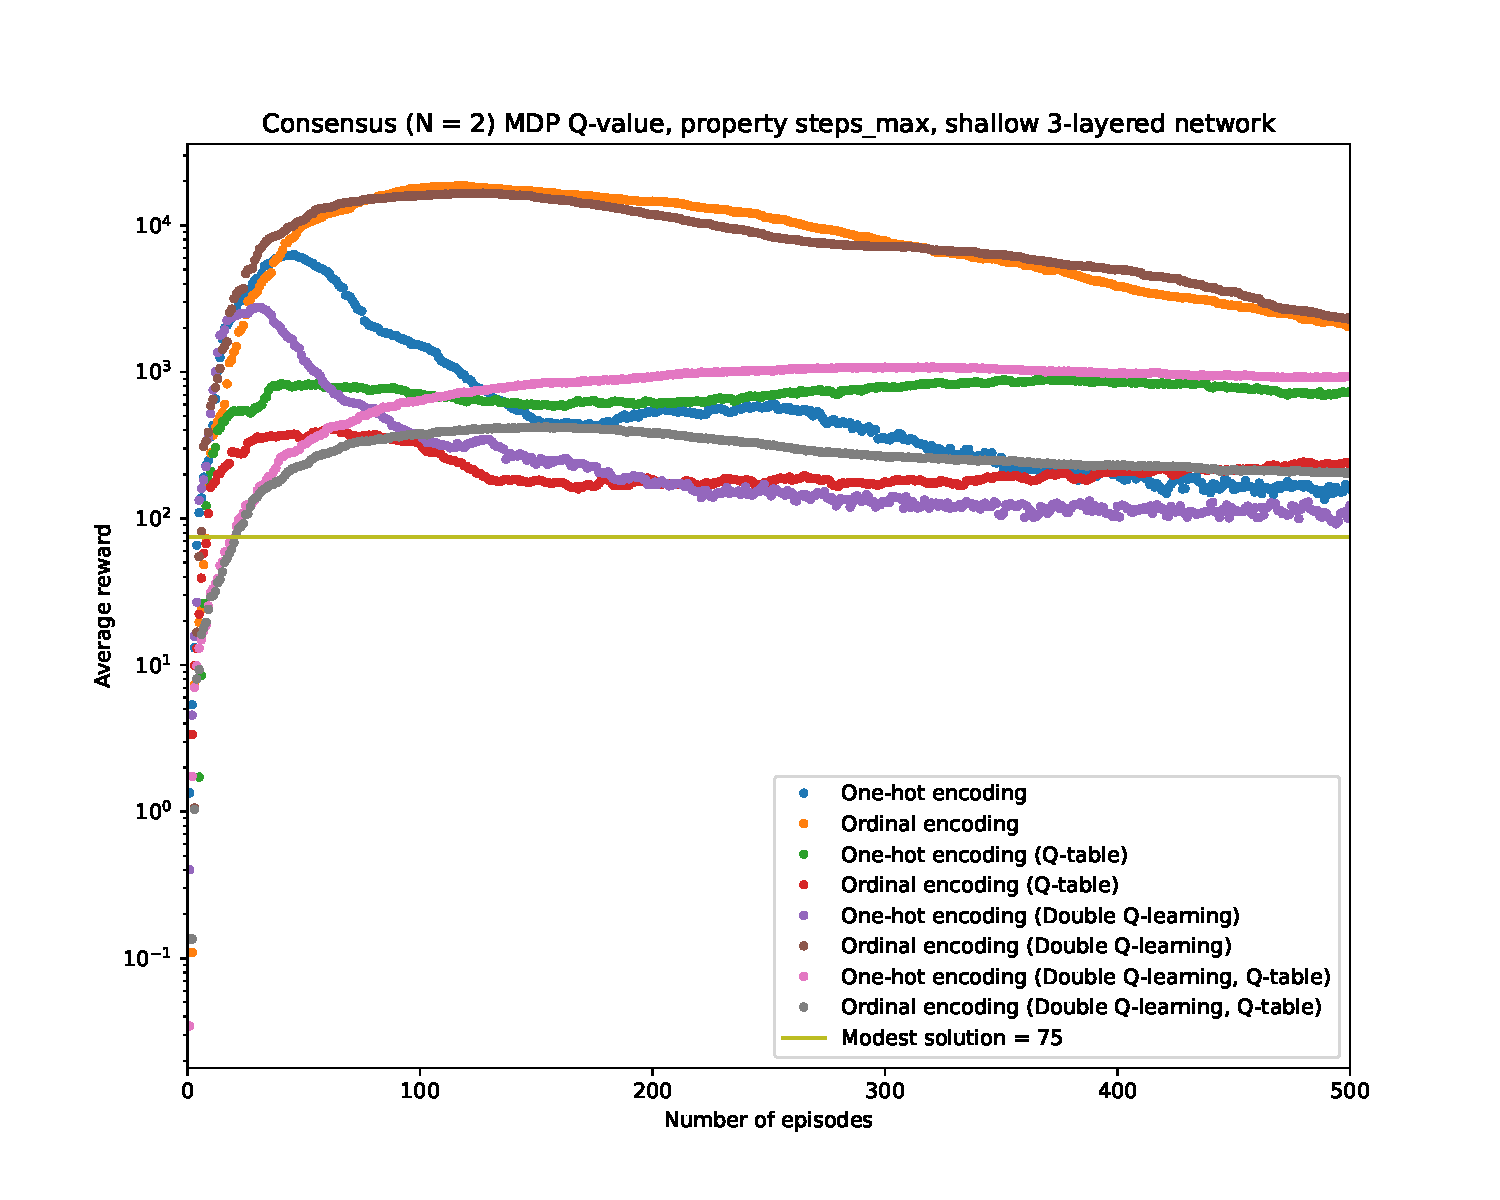
\includegraphics[width=\textwidth]{plot/consensus.2-steps_max-fc128-q.pdf}
        \caption{Consensus trained on the shallow model.}
        \label{fig:consensus.2-steps_max-shallow-q}
    \end{subfigure}
    \caption{Randomized Consensus Protocol QComp model trained on the deep and shallow network. All approaches fail to converge to or oscillate around the solution of $r = 75$.}
    \label{fig:consensus.2-steps_max-q}
\end{figure}

Figure \ref{fig:consensus.2-steps_max-q} shows not one of the approaches is able to converge to the correct solution of $r = 75$. The one-hot input-layer and Q-table approaches are the methods which get closest to the actual answer. However they are still off, and the input-layer Q-value periodically explodes in value and the Q-table approach strays further from the answer as the training continues. This holds for the deep as well as the shallow neural network, none of the approaches produced reliable results for this particular model. For this model, more complex variants were not considered for evaluation.